\documentclass[tcc2]{classe_uftex/uftex}
% ---- Esse comando cria o nome uftex estilizado
\newcommand\uftex{UF\TeX}

\usepackage{tabularx}
\usepackage{amsmath}
\usepackage{pdfpages}
\usepackage{longtable} % To display tables on several pages
\usepackage{color, colortbl}
\definecolor{Gray}{gray}{0.9}
\definecolor{LightCyan}{rgb}{0.88,1,1}
\usepackage{lipsum}
\usepackage{tikz}
\usepackage[siunitx]{circuitikz}
\usetikzlibrary{arrows}

\usepackage[alf,abnt-emphasize=bf]{abntex2cite}
\renewcommand{\backrefpagesname}{}
\renewcommand{\backref}{}
\renewcommand*{\backrefalt}[4]{}
% ----  Esse comandos são necessário no pré-ambulo para a impressão da lista de abreviaturas e de símbolos
\makelosymbols
\makeloabbreviations
% ---- Início do documento
\begin{document}
  % ---- Descrição do título do trabalho 
  \title{Descoberta de Conhecimento em Bases de Dados de Fungos da Universidade Federal do Tocantins}
  % ---- Nome do autor ou autores do trabalho
  \author{Johnny}{Gomes Pereira}
  % ---- Nome do orientador do trabalho. O último campo representa o título do professor
  \advisor{Prof.}{Ary}{Henrique Morais de Oliveira}{Dr.}
  \advisor{Profa.}{Glenda}{Michele Botelho}{Drª.}

  \examiner{Prof.}{Dr.}{Ary Henrique Morais de Oliveira}
  \examiner{Profa.}{Dra.}{Paula Benevides de Morais}
  \examiner{Prof.}{Dr.}{Wosley da Costa Arruda}
  % ---- Departamento representa o curso ao qual o trabalho está sendo apresentado. Descrito por meio de duas iniciais do curso
  \department{CC}
  % ---- Data da apresentação do trabalho
  \date{12}{07}{2020}
  % ---- Palavras-chaves em português do trabalho
  \keyword{Descoberta de Conhecimento}
  \keyword{Mineração de Dados}
  \keyword{Fungos}
  % ---- Palavras-chaves em inglês do trabalho
  \foreignkeyword{Knowledge Discovery}
  \foreignkeyword{Data Mining}
  \foreignkeyword{Fungi}
  % ---- Comando responsável por criar a capa do trabalho e/ou folha de resto conforme a configuração exigida
  \maketitle

  \frontmatter

  % ----------------------------------------------------------------------------------------------------- %
  %  Este trecho deve ser inserido somente no caso do TCC2 já na versão FINAL
  % ----------------------------------------------------------------------------------------------------- %
%   
\includepdf{ficha_catalografica}
%   
\includepdf{ata_de_aprovacao}
  % ----------------------------------------------------------------------------------------------------- %
  \dedication{A minha família, em especial aos meus pais: Olívia Gomes da Silva e Miguel Pereira da Silva - (in memoriam)}

  \begin{acknowledgement}
   A todos que contribuíram direta ou indiretamente com esta jornada. A família Arruda que me sustentou com paciência até aqui. A minha família e entes queridos pelo apoio e a todos os colegas e professores que sempre ajudaram nos momentos de dificuldade.
   Agradeço especialmente aos professores que trabalharam neste projeto: meu orientador, professor Ary Henrique Morais de Oliveira, minha coorientadora e a professora Glenda Michele Botelho, pelo tempo e dedicação que empregaram. E a professora Paula Benevides de Morais que também contribuiu com tempo, conhecimento e gentileza. 
   Agradeço ás técnicas de laboratório do LAMBIO: Cristiane e Márcia, que me auxiliaram em muitas questões de microbiologia e assim como Stella Costa, que também contribuiu com respostas a dúvidas sobre fungos leveduriformes.
   Aos amigos, Adélia Fonseca, cuja contribuição a essa jornada foi muito maior que imagina. Só tenho agradecimentos, orgulho e admiração por uma amiga assim. Ao irmão de batalhas Eufrázio Alexandre. A Jéssica Santos, Linnek Araújo, Pedro Neto Rodrigues, Renê Coutinho, Reinaldo Ribeiro e Wanderson Maior. Admiro cada um de vocês.
   Aos amigos de estágio: da Embrapa Pesca e Aquicultura e da BRK Ambiental. As experiências vivenciadas ali marcaram minha vida.
   A todos os amigos da Universidade Federal do Tocantins, sem palavras para agradecer tanta gentileza. 
   Aos familiares, em especial meus primos: Jucélio Santos e Jorlan Santos. Ao meu irmão Gabriel Gomes Pereira e a minha mãe, dona Olívia Gomes da Silva, que sempre me incentivou e superou todas as dificuldades para que eu estivesse aqui. A todos vocês meu muito obrigado. E vamos terminar logo essa graduação pelo amor de Deus.
  \end{acknowledgement}

  \begin{abstract}
  Os fungos são organismos que por anos foram classificados como plantas. Entretanto, esses possuem características tão peculiares que são hoje agrupados em um reino específico denominado Reino \emph{Fungi}. Considerando a importância dos fungos já descobertos e a imensa quantidade ainda por catalogar, este trabalho visa estudar características de fungos encontrados em frutos de Buriti e folhas de Babaçu, na região dos estados do Tocantins e Mato Grosso coletados pelo Laboratório de Microbiologia Ambiental e Biotecnologia da Universidade Federal do Tocantins. Tal estudo tem por objetivo aplicar técnicas e procedimentos de descoberta de conhecimento útil e compreensível a partir da aplicação iterativa e interativa da metodologia KDD. Dessa forma, expõe-se aqui algumas das fases do processo KDD sob a percepção de que este é amplamente utilizado pela comunidade acadêmica.
  \end{abstract}

  \begin{foreignabstract}
    % TODO: Refazer tradução e adaptação. A tradução oferecida pelo Google Translator não obteve a essência do que está escrito em português.
  \end{foreignabstract}
  \printlosymbols  
  \printloabbreviations
  % ---- Cria a lista de figuras. OPCIONAL
  \listoffigures
  % ---- Cria a lista de tabelas. OPCIONAL
  \listoftables 
  % ---- Cria o sumário. OBRIGATÓRIO
  \tableofcontents % sumário
% --- Marca o inicio dos elementos textuais. Capítulos.
\mainmatter
% ---- Defino o espaçamento de um e meio centímetros
\onehalfspacing


% --------------------------- %
% Capitulo 01: Introducao
% --------------------------- %
\ChapterStart{first}{First chapter}
\chapter{Introdução}
\label{cap:introducao}
Os fungos são organismos que por anos foram classificados como plantas% citar o trabalho de Whitetaker.
. Entretanto esses organismos, possuem características tão peculiares que são hoje agrupados em um reino á parte: o Reino \emph{Fungi}. Considerando a importância dos fungos já descobertos e a imensa quantidade ainda por catalogar, este trabalho visa estudar características de fungos encontrados em frutos de buriti e folhas de babaçu, na região dos estados do Tocantins e Mato Grosso. Tal estudo tem por objetivo aplicar técnicas e procedimentos de descoberta de conhecimento útil e compreensível a partir da aplicação iterativa da metodologia \emph{KDD}. %Dessa forma, expõe-se algumas das fases do processo \emph{KDD} sob a percepção de que este é amplamente utilizado pela comunidade acadêmica.

Através do Projeto de Pesquisa Ecologia e Bioprospecção de Fungos Mutualistas e Insetos Aquáticos em Ecossistemas Amazônicos, aprovado no Edital CNPq Redes Regionais de Pesquisa em Biodiversidade e Biotecnologia Nº 79/2013, a professora Drª Paula Benevides de Morais, coordenadora do mesmo, disponibilizou uma base de dados de fungos encontrados em frutos de Buriti (\emph{Mauritia flexuosa}) e em folhas de Babaçu (\emph{Attalea speciosa}), especificamente nas regiões dos estados do Tocantins e Mato Grosso (ver Figura \ref{fig:fig005}). Uma vez que essa base foi cedida ao Grupo de Pesquisa em Computação Aplicada do Curso de Ciência da Computação - UFT decidiu-se pela aplicação da metodologia \emph{KDD} para estudo e descoberta de conhecimento na mesma.% TODO: e o LAMBIO (Laboratório de Microbiologia Ambiental e Biotecnologia da Universidade Federal do Tocantins), ficou onde? Adicionar essa informação

    \begin{figure}[hbt]
    \centering
      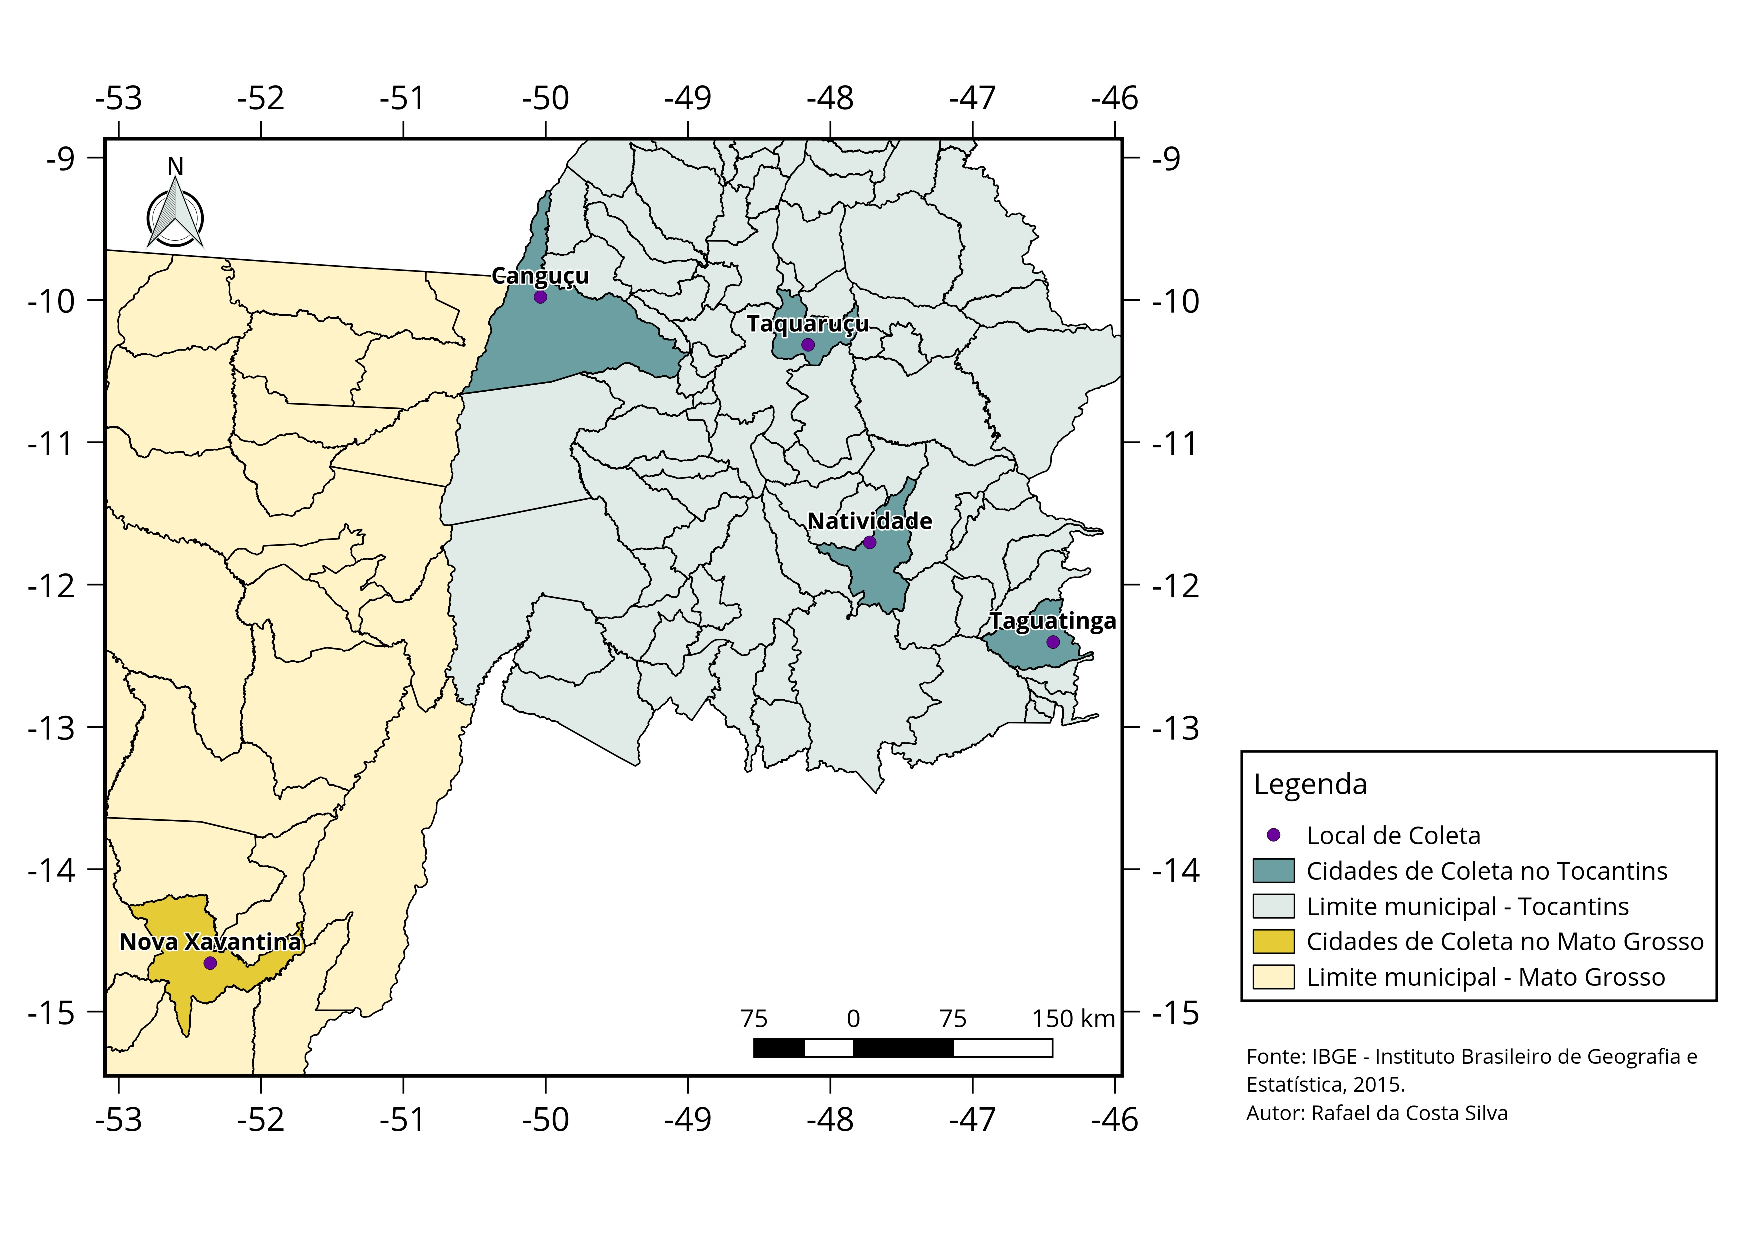
\includegraphics[scale=0.5]{TCC_Johnny/pdf/mapa_coleta.pdf}
      \caption{Locais de coleta dos fungos observados nesta pesquisa}
      %\raggedright \scriptsize \centering  Fonte: do Autor
      \label{fig:fig005}
    \end{figure}

As amostras registradas na base cedida foram retiradas de frutos de buriti e palha de babaçu. O buriti é uma palmeira de origem amazônica, típica de terrenos baixos alagáveis, igarapés e margens de rios \cite{2018:Ferreira}, seu fruto e palmito são comestíveis e a folha pode ser usada como cobertura para casas ou fibras para artesanato. Já o babaçú, é uma palmeira encontrada em regiões de clima tropical, também comum na região amazônica e Brasil central. Esta produz nozes usadas como alimento, componente para fabricação de remédios, entre outros \cite{babcu:babcu}. 

Assim, tendo em vista a importância dessas plantas bem como das comunidades de fungos que nelas se encontram, decidiu-se realizar uma pesquisa com foco na Descoberta de Conhecimento através das técnicas de mineração de dados sobre os dados fornecidos.
% TODO: Contextualizar os substratos com as comunidades de fungos neles encontrados e as características espaciais das regiões de coleta. Esse parágrafo convergirá para o contexto da biodiversidade.


\section{Justificativa}
\label{sec:justificativa}
% importância, viabilidade e oportunidade
A necessidade de registrar, recuperar e analisar dados cresce á medida que o volume de dados aumenta. O fato de diferentes pessoas se encarregarem de registrar esses dados também impacta no que se refere a consistência e integridade destes. O Laboratório de Microbiologia Ambiental e Biotecnologia (LAMBIO/UFT), registra culturas de leveduras, fungos e bactérias sem contudo, possuir uma aplicação que permita recuperar, relacionar e/ou estudar esses registros. Assim, apesar de possuir informações de fungos de diversos projetos, coletados em diferentes partes do país, em diferentes intervalos de tempo, o laboratório ainda não possui uma aplicação computacional para gerenciar ou relacionar esses dados.

A análise da base de dados de fungos através de métodos de mineração de dados pode identificar grupos de fungos com comportamentos similares que compartilham características semelhantes e que não haviam sido observados sob essa ótica de agrupamentos. É possível que existam associações que não são perceptíveis sem o auxílio da análise computacional. Uma vez que a padronização e normalização dos registros permite uma recuperação e análise inteligente desses dados, objetiva-se a criação de uma base integrada, padronizada e gerenciável pelos pesquisadores/laboratoristas de forma que estes consigam registrar, recuperar e relacionar os dados salvos em uma plataforma única. Entretanto, registrar e recuperar os dados não é suficiente pois é necessário que exista algoritmo capaz de computar índices de similaridades entre as entidades registradas em relação a comportamento, época de coleta, localização geográfica, substrato\footnote{meio de onde a amostra foi retirada, nesse caso: frutos de buriti e palhas de babaçu}, temperatura e outras variáveis.

Assim, uma vez que o Laboratório de Microbiologia Ambiental e Biotecnologia (LAMBIO/UFT), tenha um sistema capaz de gerenciar esses registros e computar esses índices de similaridades, os pesquisadores poderão desenvolver pesquisas direcionadas a grupos de comunidades específicas de fungos, de forma a integrar suas pesquisas a trabalhos em diferentes áreas.

\section{Problema}
\label{sec:problema}
Este trabalho de pesquisa visa responder as seguintes perguntas com o uso da aplicação da metodologia de descoberta de conhecimento a partir de uma base de dados integrada com informações sobre leveduras coletadas nos estados do Tocantins e Mato Grosso a fim de obter conhecimento novo, interessante, útil e aplicável. É possível agrupar os fungos dessa base de dados a partir de alguma característica em comum? 

\section{Objetivos}
\label{sec:objetivos}
    \subsection{Objetivo Geral}
    \label{subsec:objetivo_geral}
    Realizar o processo de descoberta de conhecimento em uma base de dados de fungos com o intuito de encontrar informações interessantes e úteis e modelar uma base de dados utilizando os conceitos de diagrama Entidade-Relacionamento para padronização dos dados utilizados. Para isso, os seguintes objetivos específicos precisam ser atendidos:
    
    \subsection{Objetivos Específicos}
    \label{sec:objetivos_especificos}
        \begin{enumerate}
            \item Estudar fungos, suas características e importância para a biodiversidade de forma a extrair dados importantes para o desenvolvimento do trabalho.
            \item Aplicar métodos estatísticos de análise exploratória de dados para a realização da etapa de pré-processamento, incorporando a limpeza, transformação, sumarização e integração dos dados.
            \item Estudar e aplicar técnicas de Mineração de Dados sobre a base de dados de Fungos do Laboratório de Microbiologia Ambiental e Biotecnologia da UFT;
        	\item Aplicar o processo de Descoberta de Conhecimento em Bases de Dados, ao realizar as etapas de pré-processamento, mineração de dados e pós-processamento na base de dados de fungos por meio da tarefa de mineração mais adequada ao contexto de estudos;
        	\item Modelar banco de dados relacional a fim de estruturar os dados utilizados nesta pesquisa a partir das fichas de coleta e planilhas eletrônicas utilizadas no Laboratório de Microbiologia Ambiental e Biotecnologia da UFT;
        	\item Criar um mecanismo de apresentação das informações sobre as coletas de fungos realizadas pelo Laboratório de Microbiologia Ambiental e Biotecnologia com destaque na caracterização das espécies, geolocalização de coletas e informações temporais;
        	\item Validar os resultados da mineração de dados com especialista de acordo com requisitos elencados a partir da base de dados de coleta, projetada para a execução do projeto.
        \end{enumerate}

\section{Hipóteses}
\label{sec:hipotese}
O Laboratório de Microbiologia Ambiental e Biotecnologia (LAMBIO/UFT), possui uma vasta base de dados de fungos coletados dentro e fora do estado do Tocantins por um longo período de tempo. Atualmente esses dados encontram-se registrados em planilhas eletrônicas e fichas impressas. Esses documentos contêm informações sobre: localização da coleta, substrato, datas, informações genéticas, taxonomia, reação a diversos compostos entre outras. Assim, a partir das informações disponibilizadas pelo LAMBIO/UFT, pode-se levantar as seguintes hipóteses:

    \begin{itemize}
        \item H1: É possível estabelecer relações entre fungos coletados na mesma localidade? E entre fungos coletados em localidades diferentes, é possível caracterizar essa diferenças e/ou semelhanças?
        \item H2: É possível agrupar esses fungos por alguma característica semelhante?
        \item H3: A partir das características espaciais e fisiológicas dos fungos, é possível verificar comportamentos semelhantes em reações a determinados compostos? % compostos orgânicos
        \item H4: Sobre a diversidade dos fungos catalogados pelo LAMBIO/UFT, quantos/quais destes ainda não possuem registro em coleções internacionais de cultura? Quais características proeminentes destes e como correlacioná-los ao meio em que vivem? % TODO: confirmar com especialista do contrário, remover.
    \end{itemize}


% --------------------------- %
% Capitulo 02: Fungos
% --------------------------- %
\chapter{Fungos}
\label{cap:fungos}
% classificação, diversidade, taxonomia
Conhecidos por sua capacidade de sobreviver a partir da alimentação de matéria orgânica, os fungos (que não realizam fotossíntese como as plantas) produzem enzimas que auxiliam na obtenção de minerais que provêm de plantas, animais ou outros. Estão em todos os lugares, podendo ser macroscópicos, representados pelos cogumelos ou microscópicos, subdivididos entre leveduras e bolores. No caso das leveduras, trata-se de fungos unicelulares, classificados de acordo com a morfologia ou fisiologia (Figura \ref{fig:fig007}). Eles se alimentam através da decomposição de outros seres ou mesmo interagem com eles harmoniosamente através de relação de mutualismo entre fungos e vegetais \cite{2008:Peay}. Segundo \citeonline{2016:Hibbett}, ainda há muitas espécies de fungos a serem catalogadas e estudadas.

    \begin{figure}[ht]
    \centering
      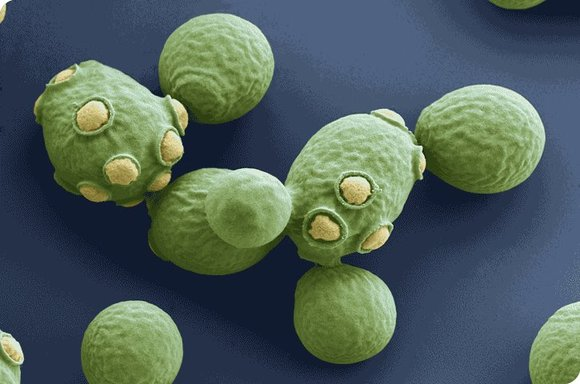
\includegraphics[scale=0.4]{TCC_Johnny/img/lev_brotamento.jpg}
      \caption{Representação de \emph{Saccharomyces cerevisiae} em brotamento.}
       \raggedright \scriptsize \centering Fonte: \citeonline{2019:micro}
      \label{fig:fig007}
    \end{figure} % TODO: trocar por uma imagem melhor

% \section{Filogenia}
% \label{sec:filogenia}
% professora Paula Benevides disse que essa pesquisa não abordará estudos em filogenia. Desconsiderar essa seção?
Alguns fungos são classificados/agrupados segundo estudos de filogenia. \citeonline{2017:Tortora} assim como \citeonline{2016:Madigan} definem filogenia como o estudo da história evolutiva dos organismos. A diversidade filogenética ainda lida com as classificações de filo, gênero e espécie á luz da evolução genética. Essa sistemática utiliza-se de termos comuns, geralmente em latim, ou grego latinizado para nomear as classes e categorias.%\footnote{Ver definição de taxa ou táxons no Dicionário de Microbiologia no apêndice}.

\section{Taxonomia}
\label{sec:taxonomia}
% TODO: responder explicitamente: Qual a diferença entre taxonomia e filogenia?
% TODO: Casar todos esses subtópicos com (bio)diversidade microbiana ou especificamente de fungos [Brock - pag 07 - cap 01]
% associar com cap 10 Tortora: Classificação dos microrganismos.
A taxonomia é a ciência que trata de arranjar ordenadamente os seres vivos \cite{2017:Tortora}. Esta,  preocupa-se com a classificação dos seres em categorias, ou seja, como esses podem ter características semelhantes (grau de similaridade) o suficiente para serem ditos de um mesmo grupo e distintos o suficientes dos seres vivos dos demais grupos. Dessa forma, é possível classificar hierarquicamente um novo indivíduo a partir das características comuns que este apresenta em relação a determinados organismos já classificados anteriormente. Atualmente tal classificação conta com auxílio de ferramentas de biologia molecular e genética para uma descrição mais precisa das características dos organismos em estudo.

Um exemplo de classificação taxonômica é visto na Figura \ref{fig:fig002}, onde é mostrada a classificação taxonômica da levedura \emph{Saccharomyces cerevisiae}, utilizada pela indústria de cerveja e na produção de pães e vinhos devido sua alta capacidade de fermentação \cite{2008:Trabulsi}.
    % principal levedura utilizada em biotecnologia no mundo segundo
    % https://www.sciencedirect.com/topics/immunology-and-microbiology/saccharomyces-cerevisiae
    \begin{figure}[hbt]
    \centering
      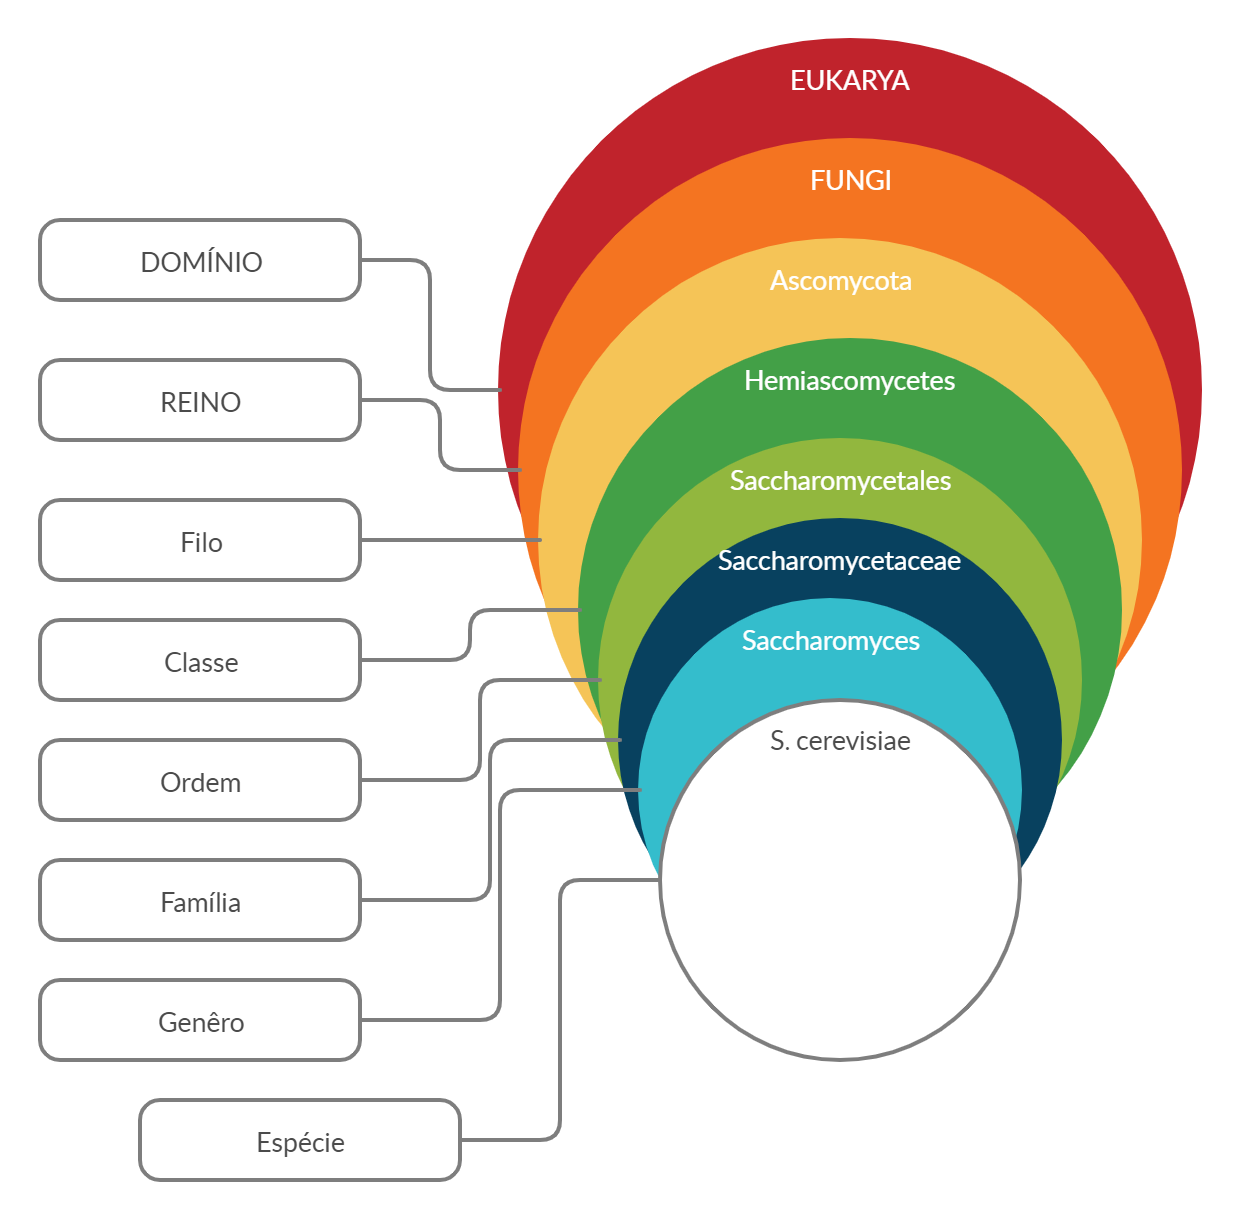
\includegraphics[scale=0.3]{TCC_Johnny/img/H_Taxonomica.png}
      \caption{Taxonomia \emph{Saccharomyces cerevisiae}.}
      \raggedright \scriptsize \centering Fonte: \citeonline{2017:Tortora}
      \label{fig:fig002}
    \end{figure} % TODO: verificar com especialista árvore taxonômica de exemplares de [genero] Candida ou Cryptococcus (pois esses que mais aparecem nas amostras da base tratada nesse trabalho)

Com o uso de informações genéticas, a partir do sequenciamento de DNA, é cada vez mais comum que a classificação filogenética reflita as relações filogenéticas \cite{2016:Madigan}. Isso implica dizer que a classificação taxonômica atual está diretamente relacionada, senão dependente, das informações filogenéticas dos indivíduos estudados.

A classificação taxonômica de um indivíduo, segundo \citeonline{2016:Madigan}, é dada seguindo a abordagem \emph{top-down} de domínio a espécie, sendo espécies similares reunidas em gêneros. Grupos de gêneros similares são reunidos em famílias. Famílias em ordens. Ordens em classes, até o domínio.

Para \citeonline{2017:Tortora}, sistemática é sinônimo de filogenia. Entretanto, para \citeonline{2016:Madigan} a sistemática relaciona filogenia á taxonomia, sendo definido como o estudo da diversidade dos organismos e suas relações. Para \citeonline{2008:Trabulsi} a sistemática se refere também a estudos envolvendo disciplinas como: morfologia, ecologia, epidemiologia, bioquímica, biologia molecular e fisiologia. % TODO: concluir pensamento sobre sistemática aqui

    % TODO: verificar necessidade/relevância com professora Paula Benevides:
    % \subsection{Classificação}
    % \label{subsec:classificacao}
    % ascomycotas, basidiomycota e deuteromycotas, os demais apenas mencionar
    

\section{Fisiologia}
\label{sec:fisiologia}
A fisiologia dos microrganismos, em especial dos fungos, foca principalmente na nutrição, crescimento, metabolismo, respiração e as associações destes com outros organismos como plantas, algas, animais ou outros.

    \subsection{Alimentação}
    \label{subsec:alimentacao}
    % TODO: falar dos compostos ao final
    Os fungos são conhecidos como quimiorganotróficos, ou seja, obtêm energia a partir de compostos químicos orgânicos \cite{2016:Madigan} e podem apresentar-se como aeróbicos, anaeróbicos ou anaeróbicos facultativos. Em sua maioria, são aeróbicos obrigatórios, isto é, possuem a necessidade de respiração. Entretanto, algumas leveduras fermentadoras são anaeróbicas facultativas, o que significa que apesar de poderem respirar, podem sobreviver em ambientes sem oxigênio \cite{2016:Madigan}\cite{2008:Trabulsi}.
    
    Uma vez que essas leveduras se alimentam de compostos orgânicos, na tabela \ref{tab:tabela02} (vide \ref{ape:apendice}) vê-se a relação de compostos orgânicos utilizados para análise das reações de crescimento das leveduras expostas a eles.
    
    \subsection{Associações}
    \label{subsec:associacoes}
    Quanto as associações, os fungos podem ser parasitas, simbiontes ou saprófagos. Os \textbf{saprófagos} vivem de substâncias em decomposição, ou seja, matéria orgânica morta. Os \textbf{parasitas} se desenvolvem em outros organismos vivos (hospedeiros). De acordo com \citeonline{2002:Black} quase todos os seres vivos, inclusive o ser humano, são parasitados por algum tipo de fungo. Alguns fungos podem causar infecções, conhecidas como micoses. Entretanto, como cita \citeonline{2010:Shaechter} muitos fungos vivem no trato gastrointestinal humano e outros revestimentos de membranas mucosas, além de serem encontrados também na pele, sob a face e couro cabeludo, sem contudo representarem riscos a saúde dos hospedeiros. Por fim, os \textbf{simbiontes} associam-se com outros organismos através de relações de mutualismo.
    
\section{Reprodução}
\label{sec:reproducao}
Para o caso das leveduras que reproduzem-se assexuadamente, é comum que estas sobrevivam a meios com pouco ou nenhum oxigênio. Já para os fungos de reprodução sexuada, a reprodução acontece apenas em ambientes ricos em oxigênio. Outra característica das leveduras é que o processo de reprodução dá-se por brotamento, ou seja, como estes microrganismos são unicelulares, sua reprodução ocorre através da criação de um nova célula de forma assexuada, deixando na célula-mãe protuberâncias que indicam que dali saíram novas células, como visto na Figura \ref{fig:fig007} que trata-se de uma representação das leveduras de \emph{Saccharomyces cerevisiae} utilizada na literatura como exemplificação de taxonomia, reprodução e fisiologia.


% \section{Ecologia e Biodiversidade}
% \label{sec:biodiversidade}
% TODO: Definir ecologia
% TODO: Definir habitat
% TODO: Definir nicho
% TODO: Contextualizar biodiversidade e participação/importância das comunidades fúngicas para manutenção dessa

% --------------------------- %
% Capitulo 03: Knowledge Discovery in Databases - KDD
% --------------------------- %
\chapter{Descoberta de Conhecimento em Bases de Dados}
\label{cap:kdd}
% historia, evolucao, secao - mineracao; tecnicas, etc...
De acordo com \citeonline{1996:Fayyad}, o termo Descoberta de Conhecimento em Bases de Dados foi cunhado em 1989 no primeiro \emph{Workshop KDD}. Esse processo, chamado simplesmente de \emph{KDD} (do inglês \emph{Knowledge Discovery in Databases}), pode ser definido como um conjunto de teorias e ferramentas para auxiliar pessoas com a extração de conhecimento válido, novo, compreensível e potencialmente útil, a partir de grandes volumes de dados \cite{1996:Fayyad}. Interessante destacar que o \emph{KDD} preocupa-se com todo o processo de descoberta de conhecimento, isto é, desde a compreensão do domínio da aplicação, a seleção, limpeza e transformação dos dados coletados, a forma em que são armazenados, selecionados, processados e transformados para então, realizar a aplicação das técnicas de mineração de dados para encontrar padrões e modelos que transformem esses dados em conhecimento. 

Outra preocupação do \emph{KDD} é que, além da preparação dos dados para aplicação do \emph{Data Mining} (ou simplesmente mineração de dados), este também estabelece  etapas bem definidas (vistas na Figura \ref{fig:fig001}) para avaliação e distribuição/implantação do conhecimento gerado nas etapas anteriores \cite{2009:Camilo}. Ou seja, minerar é importante mas, a aplicação/utilização do conhecimento é tão importante quanto.

Assim, entende-se que a Mineração de Dados consiste apenas de uma fase dentre as várias do processo de Descoberta de Conhecimento e que devido sua importância para o processo como um todo, deve possuir também etapas bem definidas. A seguir, as 9 fases da metodologia \emph{KDD} junto a uma descrição do que se pode realizar a partir do objeto dessa pesquisa: fungos unicelulares, com suas características fisiológicas e morfológicas.

     % Etapas do Processo de Descoberta de Conhecimento KDD:
    \begin{figure}[ht]
    \centering
      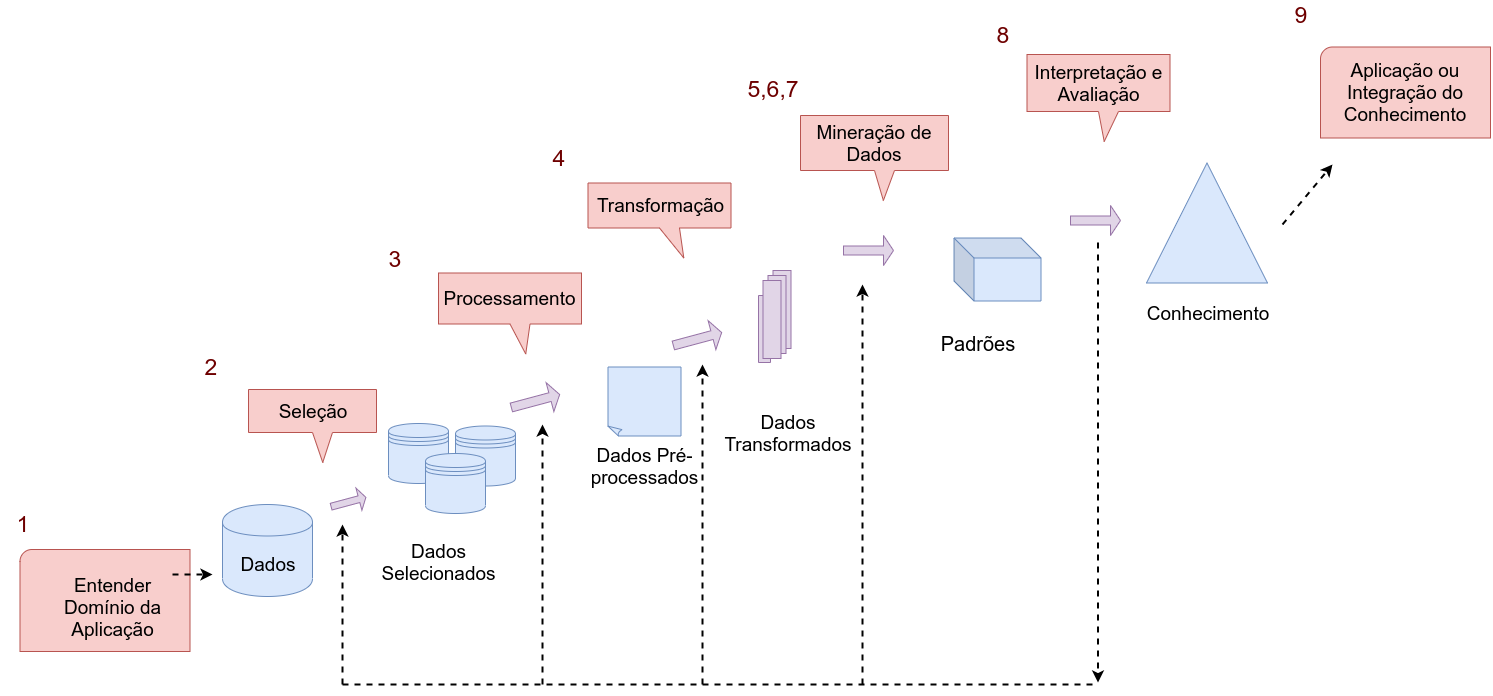
\includegraphics[scale=0.3]{TCC_Johnny/img/kdd_n.png}
      \caption{Etapas da metodologia KDD}
      \raggedright \scriptsize \centering Fonte: Adaptado de \citeonline{1996:Fayyad} e \citeonline{2014:Shafique}
      \label{fig:fig001}
    \end{figure}

\begin{enumerate}
        % Etapa 01:
        \item \emph{Entendimento do domínio da aplicação:}
        Compreender o que são fungos leveduriformes, suas características e importância para biodiversidade;
        % Etapa 02:
        \item \emph{Criação da base de dados de interesse:}
        Será utilizada a base de dados cedida pelo LAMBIO/UFT. Portanto, a relação de entidades e atributos destas, já estará contida nessa base.
        % Etapa 03:
        \item \emph{Limpeza de dados e pré processamento:}
        Realizar uma análise exploratória, utilizando métodos estatísticos. Segundo \citeonline{2009:Camilo}, alguns autores defendem que nessa fase do processo concentra-se de 50 a 80\% de todo volume de trabalho da pesquisa. Logo, essa etapa pode e deve ser considerada a principal dentre as demais. Assim \citeonline{2012:Han} define 3 subetapas que resultam no processo de entendimento dos dados:
         \begin{itemize}
             \item Limpeza dos dados:
             Eliminar problemas de registros incompletos, valores errados ou dados inconsistentes.
             \item Integração dos dados:
             Formar repositório único e consistente. Nessa etapa, será modelado e utilizado um banco de dados relacional a fim de integrar, registrar e recuperar as informações dispostas na base de dados disponibilizada pelo LAMBIO/UFT.
             \item Transformação dos dados:
             Pode-se ter necessidade de transformar valores numéricos em categóricos ou vice-versa, suavizar, sumarizar, agrupar, generalizar ou normalizar esses valores a fim de obter um modelo mais genérico ou melhor para os dados coletados.
         \end{itemize}
        % Etapa 04:
        \item \emph{Redução e Projeção de Dados:}
        Preocupa-se em encontrar atributos úteis, a depender do objetivo que se espera alcançar. Pode ser feito análise de amostragem de volume de dados sem que se perca a representatividade do mesmo.% Ver o que ocorreu com a moda das reações dos compostos que terminou por mostrar-se ineficiente para descrição dos dados uma vez que tal medida anulou a representatividade dos dados. Esses resultados são portanto, pouco relevantes para o momento e por si só não explicam muita coisa. Todavia, através dos resultados de mineração será possível cruzar essas informações com outras que talvez permitam que tais resultados se confirmem ou se confrontem no se refere a clusterização.
        % Etapa 05:
        \item \emph{Escolha das funções de mineração:}
        Está diretamente relacionado ao propósito do modelo encontrado na fase de mineração.
        % Etapa 06:
        \item \emph{Escolha dos algoritmos de mineração:}
        Os algoritmos escolhidos dependem do conhecimento que se espera obter e da forma como os dados foram tratados nas etapas anteriores. Mais detalhes no capítulo \ref{cap:metodologia}, seção \ref{sec:processamento}.
        % Etapa 07:
        \item \emph{Mineração:}
        Aplicação dos algoritmos de mineração.
        % Etapa 08:
        \item \emph{Interpretação:}
        Análise dos resultados (visualização). Testes/avaliações, correções e validações. \citeonline{1996:Silberschatz} cita que existem métricas para avaliar o quanto determinado padrão descoberto pode ser interessante para determinado problema. Essas métricas são utilizadas na etapa de pós-processamento e podem contar com participação ativa do especialista (utilização de heurística) ou apenas dos dados por si só \cite{2008:Calil}. Detalhes no capítulo \ref{cap:metodologia}, seção \ref{sec:pos_processamento}.
        % Etapa 09:
        \item \emph{Utilização do conhecimento descoberto:}
        Aplicação/utilização ou difusão do conhecimento obtido;
    \end{enumerate}
    
Importante destacar que as etapas do processo de Descoberta de Conhecimento são interativas e iterativas, ou seja, estão intrinsecamente interligadas e podem/devem se repetir ao longo da pesquisa até que se obtenham resultados satisfatórios.% TODO: Finalizar/concluir texto base.


% --------------------------- %
% Capitulo 04: Metodologia
% --------------------------- %
\chapter{Metodologia}
\label{cap:metodologia}
% aplicação da metodologia KDD na base de fungos (capítulo KDD união com capítulo Fungos em contraste com Introdução)
% TODO: Sobre as leveduras da coleção de dados, escrever visão geral passando por todas as características pertinentes citadas no capitulo de fungos

\section{Pré-Processamento dos Dados}
\label{sec:pre_processamento}
% Fases: 1 - Entendimento do domínio da aplicação
%        2 - Seleção
%        3 - Limpeza e Pré-Processamento
%        4 - Transformação

% 1 - Entendimento do domínio da aplicação
\subsection{Entendimento do domínio da aplicação}
\label{subsec:entendimento_dominio}
O Laboratório de Microbiologia Ambiental e Biotecnologia da Universidade Federal do Tocantins (LAMBIO/UFT) trabalha com coleções de culturas de bactérias, fungos e leveduras. Geralmente os dados das amostras coletadas são registradas em arquivo impresso ou planilhas eletrônicas. Nesse arquivo é registrado o projeto a qual pertence aquela amostra, dados do local de coleta, dados do responsável pela coleta, substrato, a data da realização da coleta, e dá-se um código único para identificação daquela amostra (também chamado de isolado). Esses são identificadores da amostra e vão no cabeçalho do arquivo impresso, ou nas primeiras abas da planilha eletrônica. Para os casos de registros de amostras de leveduras, é registrado fonte de isolamento, variedade, meio de cultivo e espécie. Na sequência, são registradas as características morfológicas das leveduras: elevação, borda, cor, aspecto, brotamento e um campo onde o pesquisador/laboratorista pode registrar a descrição colonial. Após isso, são registradas as características morfológicas relacionadas á reprodução dos fungos, através do preenchimento de dados categóricos para esporos, que podem ser sexuais ou assexuais, com a descrição de forma e número.

     % Disposição dos dados em planilha eletrônica, com reação de leveduras a determinados compostos:
    \begin{figure}[ht]
    \centering
      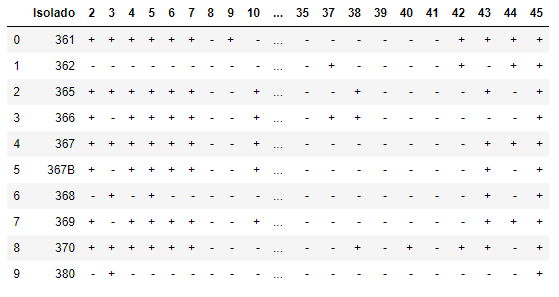
\includegraphics[scale=0.9]{TCC_Johnny/img/reacao_composto.PNG}
      \caption{Disposição dos dados em planilha eletrônica.}
      \raggedright \scriptsize \centering Fonte: Adaptado da Base de Dados LAMBIO/UFT
      \label{fig:fig008}
    \end{figure}

Por fim, há uma tabela para descrição fisiológica dessas leveduras. Nessa tabela estão dispostos os compostos orgânicos vistos na Tabela de Compostos (Apêndice \ref{ape:apendice}), com seus respectivos números de identificação. Á frente de cada composto, três colunas onde o pesquisador/laboratorista deve registrar a reação da levedura àquele composto. Os campos de reações devem ser marcados com os seguintes símbolos padronizados pelo LAMBIO/UFT: \emph{-, *, +}\footnote{nas planilhas eletrônicas encontrou-se também os marcadores \emph{w, W, s, S, NR, NC} que basicamente indicam reações similares aos marcadores principais sendo portanto, substituídos pelos mesmos.} (ver descrição dos marcadores na Tabela \ref{tab:tabela03}). A observação das reações é registrada a cada sete dias e portanto, a primeira coluna é preenchida no sétimo dia após a exposição da levedura, a segunda no décimo quarto e a terceira coluna no vigésimo primeiro dia de exposição. Uma vez com os três registros das reações, o pesquisador/laboratorista deverá então registrar a combinação desses marcadores em uma quarta coluna contendo o resultado final da reação da levedura ao composto em observação (vide Figura \ref{fig:fig008}). É essa coluna com o resultado final que é levada em consideração para as análises de comportamento de leveduras nas pesquisas do LAMBIO/UFT. Outra ficha utilizada pelo Laboratório tem o objetivo de registrar o comportamento dessas leveduras quanto á relação de variação de temperatura e a fermentação (Apêndice \ref{ape:fichas}).

    \begin{table}%[h!]
    \centering
    \caption{\label{tab:tabela03} Marcadores para sinalizar as reações }
    \begin{tabular}[c]{rl}
    \hline
     \textbf{Marcador} & \textbf{Descrição} \\
     \hline
        \textbf{+} & indica crescimento a partir da exposição ao composto \\
        \textbf{*} & indica que a amostra não apresentou crescimento significativo \\
        \textbf{-} & indica decrescimento da amostra ao ser exposta ao composto \\
      \hline
     \raggedright \scriptsize \centering Fonte: do Autor
    \end{tabular}
    \end{table}
    

% 1.1 Descrição dos dados:
    \subsection{Entendimento dos dados}
    \label{subsec:entendimento_dados}
    Diferente da metodologia CRISP-DM 1.0, a metodologia KDD, divide a fase de Entendimento dos dados em duas: \emph{2 - Criação da base de dados de interesse} e \emph{3 - Limpeza de dados e pré-processamento}. Assim, seguindo a metodologia descrita por \citeonline{1996:Fayyad}, tem-se que a base de dados com suas entidades relacionadas e seus atributos já fora criada, o que permite seguir para a próxima etapa. Ao estudar os dados da base de fungos do LAMBIO/UFT, estes podem ser divididos em dois grupos principais: metadados e dados brutos (Ver diagrama Entidade Relacionamento no Apêndice \ref{ape:modelo_er}). Os primeiros contêm dados sobre o projeto da pesquisa que motivou a coleta, informações do responsável pela coleta, da localidade e do tempo. O segundo, trata do objeto da pesquisa. Neste caso, leveduras.
     
     Através das reuniões com os especialistas e leitura de material bibliográfico foi possível melhorar a compreensão do domínio e dos dados e com isso, construir um dicionário de dados sobre os atributos contendo nome, significado, tipo de dado, intervalo para valores permitidos para o atributo, descrição se este pode ser zero ou nulo, entre outros (ver Apêndice \ref{ape:dicionario}). A primeira constatação quanto á classificação dos dados diz respeito ao nível de mensuração destes. Segundo \citeonline{2011:Bonafini}, existem 4 níveis de medida, sendo: \emph{nominal}, \emph{ordinal}, \emph{intervalar} e \emph{racional}.
     
     De início, percebe-se que todos os dados da base podem ser qualificados como qualitativos nominais. O que significa que esses são categorizáveis (por isso também chamados de variáveis categóricas) não sendo possível portanto, ordená-los, estabelecer intervalos ou subtrair valores destes para fins de comparação ou mesmo determinar se um dado é múltiplo de outro. Com isso, é possível selecionar algumas técnicas de estatística descritiva em detrimento de outras com o objetivo de conhecer a distribuição e comportamento desses dados.
     
     % Subetapas da fase 03 aqui: 
     De acordo com \cite{2008:Peay}, existem 3 subetapas importantes para o processo de entendimento dos dados, a seguir a descrição do trabalho realizado em cada uma destas conforme contexto do trabalho:
     \begin{itemize}
         \item \emph{Limpeza dos dados:} Nas planilhas eletrônicas alguns registros possuem dados faltantes, como a não observação da reação a
determinado composto, ou colunas sem registro de dados. Para o momento, esses registros foram omitidos. Dessa forma, não se contabilizam reações ‘nulas’. Nesta etapa também são realizados procedimentos para detecção de \emph{outliers}, dados discrepantes originados de erros de medição/interpretação ou preenchimento. Entretanto, dado a especificidade dos dados, nada foi feito quanto a este passo. Ademais, métodos de agrupamentos Baseados em Densidade e métodos Hierárquicos são capazes de detectar dados discrepantes. % 
         \item \emph{Transformação dos dados:} Como as planilhas eletrônicas foram preenchidas por alunos diferentes, as reações aos compostos foram registradas utilizando marcadores diferentes. Assim, houve necessidade de transformar esses símbolos em números para melhor visualização gráfica da distribuição dos dados e para padronização desses marcadores. Dessa forma, a tupla \emph{(-, *, +, w, W, s, S, NR, NC)} foi substituída por \emph{(0,1,2,3,3,4,4,5,6)}. Onde antes os compostos eram identificados pelos nomes, passaram a ser identificados apenas pelo número correspondente. Os isolados/amostras passaram a ser identificadas somente pelo código no freezer, sendo descartados os números de identificação dados pelos alunos no momento da coleta. Vale ressaltar que, mesmo os marcadores sendo substituídos por números, o tipo de dado continua sendo categórico. %
         \item \emph{Integração dos dados:} A fim de manter os registros organizados, alguns alunos registraram as reações em abas distintas na mesma planilha eletrônica. Porém, como os registros possuem mesmo identificador (código do isolado) foi possível integrar essas tabelas com base nesse identificador único, uma vez que se tratam de informações sobre as mesmas entidades: a relação entre os isolados e os compostos a qual estes foram expostos. %
     \end{itemize}
     
         \begin{figure}[hbt]
         \centering
          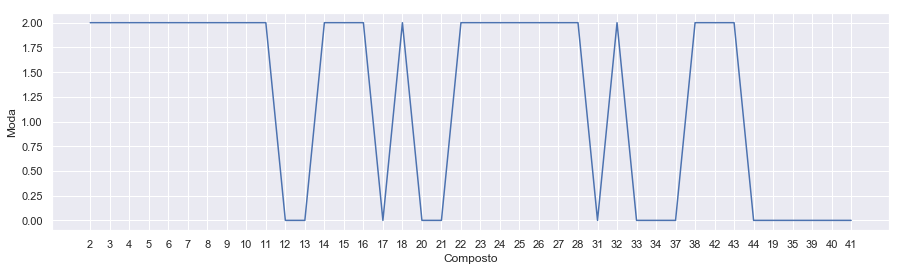
\includegraphics[scale=0.5]{TCC_Johnny/img/Babacu_Moda-reacaoComposto.png}
          \caption{Relação de Reações a determinados Compostos para Fungos de Babaçu}
          \footnotesize{Fonte: do Autor}
          \label{fig:fig003}
        \end{figure}
        
        \begin{figure}[hbt]
        \centering
          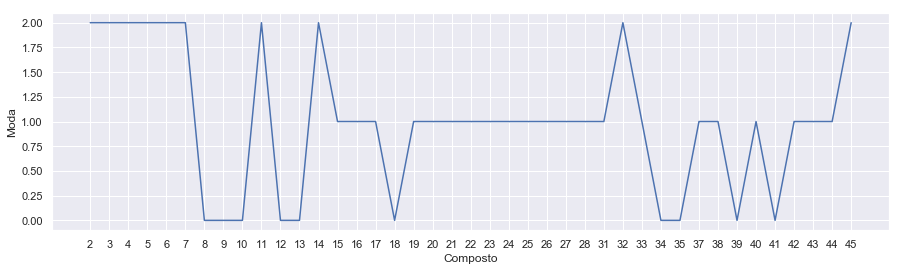
\includegraphics[scale=0.5]{TCC_Johnny/img/Buriti_Moda-reacaoComposto.png}
          \caption{Relação de Reações a determinados Compostos para Fungos de Buriti}
          \footnotesize{Fonte: do Autor}
          \label{fig:fig004}
        \end{figure}
    
    Através das técnicas de \textbf{análise exploratória}, utilizadas para busca por identificação de padrões nos dados, foi possível levantar mais informações sobre os dados da base. A análise exploratória possibilita verificar a distribuição de frequência e medidas de tendência central, como média, mediana e moda. Como os dados da base de fungos foram todos qualificados como atributos categóricos, excluem-se as medidas de média e mediana, por não serem aplicáveis a este tipo de dados. Com a aplicação da moda, medida resumo definida por \citeonline{2010:Bussab} como valor ou atributo que aparece com maior frequência, tem-se uma visão sumarizada desses dados. De acordo com os gráficos da Figura \ref{fig:fig003} e Figura \ref{fig:fig004} pode-se observar a tendência de crescimento das leveduras quando expostas aos compostos orgânicos vistos na Tabela \ref{tab:tabela02}. No gráfico da Figura \ref{fig:fig004}, vê-se que as amostras de leveduras de Buriti manifestaram predominantemente reação de crescimento quando expostas aos compostos de número 2,3,4,5,6,7,11,14,32 e 45. As mesmas decresceram quando expostas aos compostos de número 8,9,10,12,13,18,34,35,39 e 41. Por fim, vê-se que nos compostos 15,16,17,19,20,21,22,23,24,25,26,27,28,31,37,38,40,42,43 e 44 essas leveduras apresentam comportamento predominantemente estável. Vale destacar que, neste caso, a utilização de medida resumo como técnica de Redução e Projeção de dados (etapa 4) revela pouca representatividade para os mesmos. Todavia, através dos resultados de mineração será possível cruzar essas informações com outras que permitam que tais resultados se confirmem ou se confrontem á luz dos objetivos descritos no Capítulo \ref{cap:introducao}, seção \ref{sec:objetivos}.
    
    \begin{table}%[h!]
    \centering
    \caption{\label{tab:tabela01} Distribuição dos dados}
    \begin{tabular}[c]{lllrrrr}
    \hline
     \textbf{Localidade} & \textbf{UF} & \textbf{Substrato} & \textbf{Isolados} & \textbf{\%} & \textbf{Mês/Ano}\\
     \hline
    Canguçu	& TO & Babaçu & 53 & 6,9\% & - \\
    Canguçu	& TO & Buriti & 199 & 25,91\% & janeiro/2014\\
    Natividade & TO & Babaçu & 72 & 9,37\% & - \\
    Nova Xavantina & MT & Buriti & 81 & 10,55\% & agosto/2015\\
    Taguatinga & TO & Buriti & 82 & 10,67\% & janeiro/2014\\
    Taquaruçu & TO & Babaçu & 67 & 8,72\% & - \\
    Taquaruçu & TO & Buriti & 214 & 27,86\% & novembro/2014\\
      \hline
      \textbf{Total} & & & \textbf{768} \\
     %\hline
    \raggedright \scriptsize \centering Fonte: do Autor
    \end{tabular}
    \end{table}
    

\section{Processamento}
\label{sec:processamento}
% TODO: breve visão geral sobre o assunto
% Fases: 5 - Escolha das funções de mineração - R.: queremos encontrar agrupamentos
%        6 - Escolha dos algoritmos de mineração - R.: ainda não sabemos quais algoritmos utilizar
%        7 - Mineração - R.: ainda não sabemos o que vamos encontrar com a mineração
Nessa etapa do processo utilizam-se as fases \emph{5 - Escolha das funções de mineração}, \emph{6 - Escolha dos algoritmos de mineração} e \emph{7 - Mineração} da metodologia KDD. Em resposta a etapa 5, de acordo com os objetivos descritos na seção \ref{sec:objetivos}, sabe-se que as funções de mineração escolhidas serão aquelas que modelem os dados a partir de agrupamentos de forma a estabelecer relações entre elementos de um mesmo grupo e revele graus de dissimilaridade entre elementos de grupos distintos. A seguir, alguns tipos de métodos de agrupamentos que permitem a análise de objetos de dados sem consulta a classes predefinidas, apresentados como sinônimo para algoritmos de aprendizado não supervisionado \cite{2012:Han}.
    
     \subsection{Medidas de Distância e Similaridade}
     \label{subsec:medidas}% TODO: escrever breve resumo > Euclidiana, Minkowski, Manhattan... infelizmente essas só servem para dados numéricos, o que não é o caso aqui. Conforme cita \citeonline{2010:Maimon}, para dados nominais, tem-se duas medidas de distâncias, que são
    % 1 - Combinação Simples:
    % 2 - Criar atributo binário para cada estado de cada atributo nominal e e computar o grau de dissimilaridade, conforme descrito acima
    Para que os algoritmos de agrupamentos funcionem corretamente é necessário que seja definido uma boa medida de similaridade entre as instâncias \cite{2013:chapman}. As medidas de distância ou similaridade mais conhecidas são Distância Euclidiana (utilizada no K-Means), Minkowski e Manhattan \cite{2007:Omran}. Entretanto, como observado por \citeonline{1988:Jain}, essas medidas são aplicáveis somente a dados numéricos, não sendo possível aplicá-las a dados categóricos. Conforme cita \citeonline{2010:Maimon}, para dados nominais, tem-se duas medidas de distâncias, que são:
    \begin{enumerate}
        \item \emph{Combinação Simples} que consiste em comparar diretamente a estrutura dos objetos;
        \item \emph{Criar atributo binário} para cada estado de cada atributo nominal e computar o grau de dissimilaridade, conforme descrito acima;
    \end{enumerate}
    
    % Funções de similaridade: Cosine Measure, Pearson Correlation Measure, Extended Jaccard Measure, ...
    
    \subsection{Métodos de Particionamento}
    \label{subsec:particionamento}
    Este método divide o conjunto de \emph{n} objetos em \emph{k} partições nos dados de forma que cada partição represente um \emph{cluster} e \emph{k $\leqslant$ n} \cite{2012:Han}. Estes métodos realocam instâncias em movendo-as, de modo iterativo, de um \emph{cluster} para outro \cite{2010:Maimon}. Outra característica desse método é a necessidade de o usuário ter que escolher, mesmo que aleatoriamente, o número de \emph{cluster} que deseja que o método separe. Para solucionar esse problema torna-se imprescindível que o usuário entenda do domínio da aplicação e conheça os dados em que se aplica o método. O algoritmo mais conhecido dentro desse método de agrupamento é o \emph{k-means}, algoritmo que particiona os dados em \emph{k} grupos $(C_1,C_2,...,C_k)$ representados pelos centroides ou médias. O centro de cada grupo é calculado como a média das instâncias daquele grupo. Os centroides inicias podem ser escolhidos randomicamente ou baseados em alguma heurística \cite{2010:Maimon}. A cada iteração todas as instâncias são atribuídas ao centroide mais próximo de acordo com a distância euclidiana. O centroide é recalculado e tomado como novo centro do grupo. Por fim, todo o processo se repete para os novos centroides do grupo até que não haja mais novos centroides. Como vantagem cita-se o fato de que o método é dinâmico e mesmo que no início um objeto seja atribuído a um grupo errado, este ainda pode ser realocado em um grupo com maior similaridade \cite{2007:Omran}. 
        
        % \begin{equation}
        %     \mu_k = \frac{1}{N_k} \sum_{q=1}^{N_k} x_q
        %     \label{eqn:kmeans_formula}
        % \end{equation}% TODO: explicar didaticamente essa fórmula
        
        % TODO: inserir pseudo-código do k-means aqui 
     
    \subsection{Métodos de Agrupamento Hierárquico}
    \label{subsec:hierarquico}
    Um método hierárquico cria uma decomposição hierárquica do conjunto de dados. Estes podem ser classificados como sendo aglomerativos ou divisivos, com base em como a decomposição hierárquica é formada \cite{2010:Maimon}. A abordagem aglomerativa, também chamada de \emph{bottom-up}, começa com cada objeto formando um grupo separado. Ele mescla sucessivamente os objetos ou grupos próximos uns aos outros, até que todos os grupos sejam mesclados em um (o nível mais alto do hierarquia) ou que uma condição de parada seja satisfeita \cite{2012:Han}. A abordagem divisiva, também chamada de abordagem \emph{top-down}, começa com todos os objetos no mesmo \emph{cluster}. Em cada iteração, um \emph{cluster} é dividido em \emph{clusters} menores, até que, eventualmente, cada objeto esteja em um \emph{cluster} ou uma condição de parada seja satisfeita. Os métodos de agrupamento hierárquico podem ser baseados em distância ou baseados em densidade e continuidade. Várias extensões de métodos hierárquicos também consideram agrupamentos em subespaços. Como resultado, os métodos de agrupamento hierárquicos produzem uma estrutura em formato de árvore, chamada de dendograma. Estas são de fácil entendimento para o ser humano, ainda que haja um certo nível de subjetividade nos resultados \cite{1988:Jain}. Para lidar com essa subjetividade a participação de um especialista no processo de avaliação e correção auxilia a mitigar problemas e conduz a resultados mais satisfatórios. Os métodos hierárquicos sofrem com o fato de que uma vez que uma etapa (mesclagem ou divisão) é concluída, esta nunca pode ser desfeita. Essa rigidez é útil, pois leva a custos de computação menores, por não ter que se preocupar com um número diferente de opções combinatórias. Tais técnicas são estáticas, ou seja, não podem corrigir decisões erradas. Entretanto, existem métodos propostos para melhorar a qualidade do \emph{cluster} resultante.% citar exemplos, vantagens e desvantagens.
    
    \subsection{Métodos Baseados em Grade e Densidade}
    \label{subsec:densidade}% vale mesmo a pena deixar essa seção no trabalho?
    % TODO: adicionar comentários sobre métodos baseados em grade
    Métodos baseados em densidade assumem que os pontos que pertencem a cada grupo são extraídos de uma distribuição de probabilidade específica. Presume-se que a distribuição geral dos dados seja uma mistura de várias distribuições. O objetivo desses métodos é identificar os \emph{clusters} e seus parâmetros de distribuição \cite{2010:Maimon}.
    
    A ideia geral deles é continuar crescendo um determinado \emph{cluster} enquanto a densidade (número de objetos ou pontos de dados) na vizinhança excede algum limite. Por exemplo, para cada ponto de dados em um determinado \emph{cluster}, a vizinhança de um determinado raio deve conter pelo menos um número mínimo de pontos. Esse método pode ser usado para filtrar ruídos ou detectar \emph{outliers} e descobrir grupos de forma arbitrária.

\section{Pós-Processamento dos Dados}
\label{sec:pos_processamento}
% Fases: 8 - Interpretação e Avaliação
%        9 - Aplicação/difusão do conhecimento
%  destaque para representação ou apresentação do conhecimento: gráficos, relatórios, regras de associação, etc. 
Esta é a etapa final do processo e compreende as fases \emph{8 - Interpretação e Avaliação} e \emph{9 - Aplicação/difusão do conhecimento} da metodologia KDD. Por se tratar de uma metodologia interativa, a participação dos especialistas é elemento fundamental em todas as fases. Mais ainda na fase 8 pois nela, utilizar-se-á dos conhecimentos e experiência dos especialistas para que estes interpretem e avaliem os resultados obtidos. Como vantagem da utilização de uma metodologia iterativa tem-se que, caso exista necessidade de correções e/ou melhorias, o processo deverá voltar às fases anteriores e se repetirá até que se obtenha respostas satisfatórias as perguntas iniciais que levaram ao desenvolvimento do projeto.

% --------------------------- %
% Capitulo 06: Resultados
% --------------------------- %
\chapter{Resultados Esperados}
\label{cap:resultados}
Ao final deste trabalho pretende-se alcançar o Objetivo Geral proposto, passando pelos Objetivos Específicos. Encontrar as respostas para o Problema abordado e validar as Hipóteses levantadas, para isso realizando as etapas apresentadas no capítulo Metodologia.

Almeja-se encontrar agrupamentos de fungos coletados no estado do Tocantins e Mato Grosso a partir do resultados das reações destes com alguns compostos orgânicos. Esses resultados deverão ser validados pelos especialistas e por fim, será proposto modelo de agrupamento obtido através da mineração de dados, para sistema de banco de dados de informações sobre fungos coletados pelo Laboratório de Microbiologia Ambiental e Biotecnologia da Universidade Federal do Tocantins.

Assim, uma vez adquirido informações que se façam interessantes e úteis através da Descoberta de Conhecimento nessa base de dados e com um modelo de dados que permita extrair novas informações a partir de uma base padronizada o Laboratório de Biotecnologia da Universidade Federal do Tocantins poderá prosseguir com pesquisas especializadas nessas e outras descobertas permitidas pela padronização e normalização dos dados na base.


\backmatter 
\singlespacing   
% ----------------------------------------------------------------------------------------------------- %
\bibliography{TCC_Johnny}

\appendix
\onehalfspacing

\chapter{Tabela de Compostos}
\label{ape:apendice}

\begin{table}[hbt]
\caption{Tabela de Compostos}
  \label{tab:tabela02}
\begin{tabular}[c]{|l|l|l|l|l|l|}
  \hline
  \textbf{Id} & \textbf{Composto} & \textbf{Id} & \textbf{Composto} & \textbf{Id} & \textbf{Composto}\\
  \hline
    \rowcolor{LightCyan}
    0 &	YNB BRANCO & 23	& GALACTITOL	& 46	& YNB S/AA\\
    1 &	GLICOSE	& 24	& D-MANITOL	& 47	& YNB S/VIT\\
     \rowcolor{LightCyan}
    2 &	GALACTOSE	& 25	& D-GLUCITOL	& 48	& YCB\\
    3 &	L-SORBOSE	& 26	& A-M-GLICOSIDEO	& 49	& N1 - NITRATO\\
     \rowcolor{LightCyan}
    4 &	MALTOSE	& 27	& SALICINA	& 50	& N2 - NITRITO\\
    5 &	SACAROSE	& 28	& GLU-$\delta$-LACTONA	& 51	& N3 - L-LISINA\\
     \rowcolor{LightCyan}
    6 &	CELOBIOSE	& 29	& 2-K-GLUCONATO	& 52	& N4 - CADAVERINA\\
    7 &	TREALOSE	& 30	& 5-K-GLUCONATO	& 53	& N5 - ETLAMINA-HCL\\
     \rowcolor{LightCyan}
    8 &	LACTOSE	& 31	& DL-LACTATO	& 54	& D-GLUCONATO\\
    9 &	MELIBIOSE	& 32	& SUCCINATO	& 55	& PROTEASE PH 3.0\\
     \rowcolor{LightCyan}
    10 &	RAFINOSE	& 33	& CITRATO	& 56	& PROTEASE PH 5.0\\
    11 &	MELEZITOSE	& 34	& M-INOSITOL	& 57	& PROTEASE PH 7.0\\
     \rowcolor{LightCyan}
    12 &	INULINA	& 35	& METANOL	& 58	& PROTEASE PH 9.0\\
    13 &	AMIDO	& 36	& HEXADECANO	& 59	& PECTINASE\\
     \rowcolor{LightCyan}
    14 &	D-XILOSE	& 37	& GLUCOSAMINA	& 60	& AMILASE\\
    15 &	L-ARABINOSE	& 38	& XILITOL	& 61	& LIPASE\\
     \rowcolor{LightCyan}
    16 &	D-ARABINOSE	& 39	& ACETONA	& 62	& DBB\\
    17 &	D-RIBOSE	& 40	& ETILACETATO	& 63	& UREASE\\
     \rowcolor{LightCyan}
    18 &	L-RAMNOSE	& 41	& ISOPROPANOL	& 64	& C AMILÓIDES\\
    19 &	ETANOL	& 42	& GLUCONATO	& 65	& 10\% NaCl\\
     \rowcolor{LightCyan}
    20 &	GLICEROL	& 43	& NGLUCOSAMINA	& 66	& 50\% GLI\\
    21 &	ERITRITOL	& 44	& CICLOHEXIMIDA 0,01	& 67	& ACIDO\\
     \rowcolor{LightCyan}
    22 &	RIBITOL	& 45	& CICLOHEXIMIDA 0,1 &  & \\
\hline
\end{tabular}
\raggedright \scriptsize \centering Fonte: Fichas Coleção Culturas LAMBIO/UFT
\end{table}

% INSERIR: Dicionário de termos técnicos de Microbiologia
\chapter{Dicionario de Dados}
\label{ape:dicionario}

\begin{table}[hbt]
\caption{Tabela de Dicionário de Dados}
  \label{tab:tabelaD}
\begin{tabularx}{\textwidth}{l|l|l|X}
  %\hline \hline
  \toprule
  \textbf{Atributo} & \textbf{Tipo Dado} & \textbf{Nulo} & \textbf{Descrição} \\
  %\hline \hline
   \midrule
    Espécie & Categórico & Sim & Identificação taxonômica do isolado, compreende gênero, espécie,... \\
    \hline
    Variedade & Categórico & Sim & Informação relativa a identificação taxonômica (complementar) \\
    \hline
    Fonte isolamento & Categórico & Não & Meio para isolar uma espécie dos demais encontradas \\%
    \hline
    Código & Categórico & Não & Identificador da amostra no freezer do LAMBIO \\
    \hline
    Substrato &  Categórico & Não & Meio de origem da amostra: fruto, solo, planta, etc \\
    \hline
    Meio de cultivo &  Categórico & Não & Meio Utilizado para cultivar isolado de forma a mantê-lo sob observação \\%
    \hline
    Material &  Categórico & Não & Material utilizado no meio de cultivo \\%
    \hline
    Local &  Categórico & Não & Dados sobre local da coleta: País, Estado, Cidade, Região... \\
    \hline
    Data &  Categórico & Não & Dia, mês e ano da realização da Coleta \\
    \hline
    Descrição colonial & Categórico & Sim & Descrição a cargo do pesquisador/laboratorista \\
    \hline
    Elevação & Categórico & Sim & Característica intrínseca de fungo \\
    \hline
    Borda & Categórico & Sim & Característica intrínseca de fungo \\
    \hline
    Cor & Categórico & Sim & Coloração do levedura,fungo,colônia \\
    \hline
    Aspecto & Categórico & Sim & Característica intrínseca de fungo \\
    \hline
    Brotamento & Categórico & Sim & Característica intrínseca de fungo \\
    \hline
    Meio Líquido & Categórico & Sim & Meio com nutrientes para observação da fisiologia da levedura \\
    \hline
    Esporos & Categórico & Sim & Característica intrínseca de fungo \\
    \hline
    Forma & Categórico & Sim & Diretamente relacionado ao item anterior \\
    \hline
    Número & Numérico & Sim & Diretamente relacionado ao item anterior \\
    \hline
    Id Composto & Categórico & Não & Número de identificação do composto  \\
    \hline
    Composto & Categórico & Não & Descrição/nome do composto \\
    \hline
    Reação & Categórico & Sim & Campo para marcador de comportamento da levedura sob exposição a determinado composto \\%
%\hline
\bottomrule
\end{tabularx}
\raggedright \scriptsize \centering Fonte: do Autor
\end{table}

\chapter{Modelo Entidade Relacionamento}
\label{ape:modelo_er}

 \begin{figure}[ht]
    \centering
      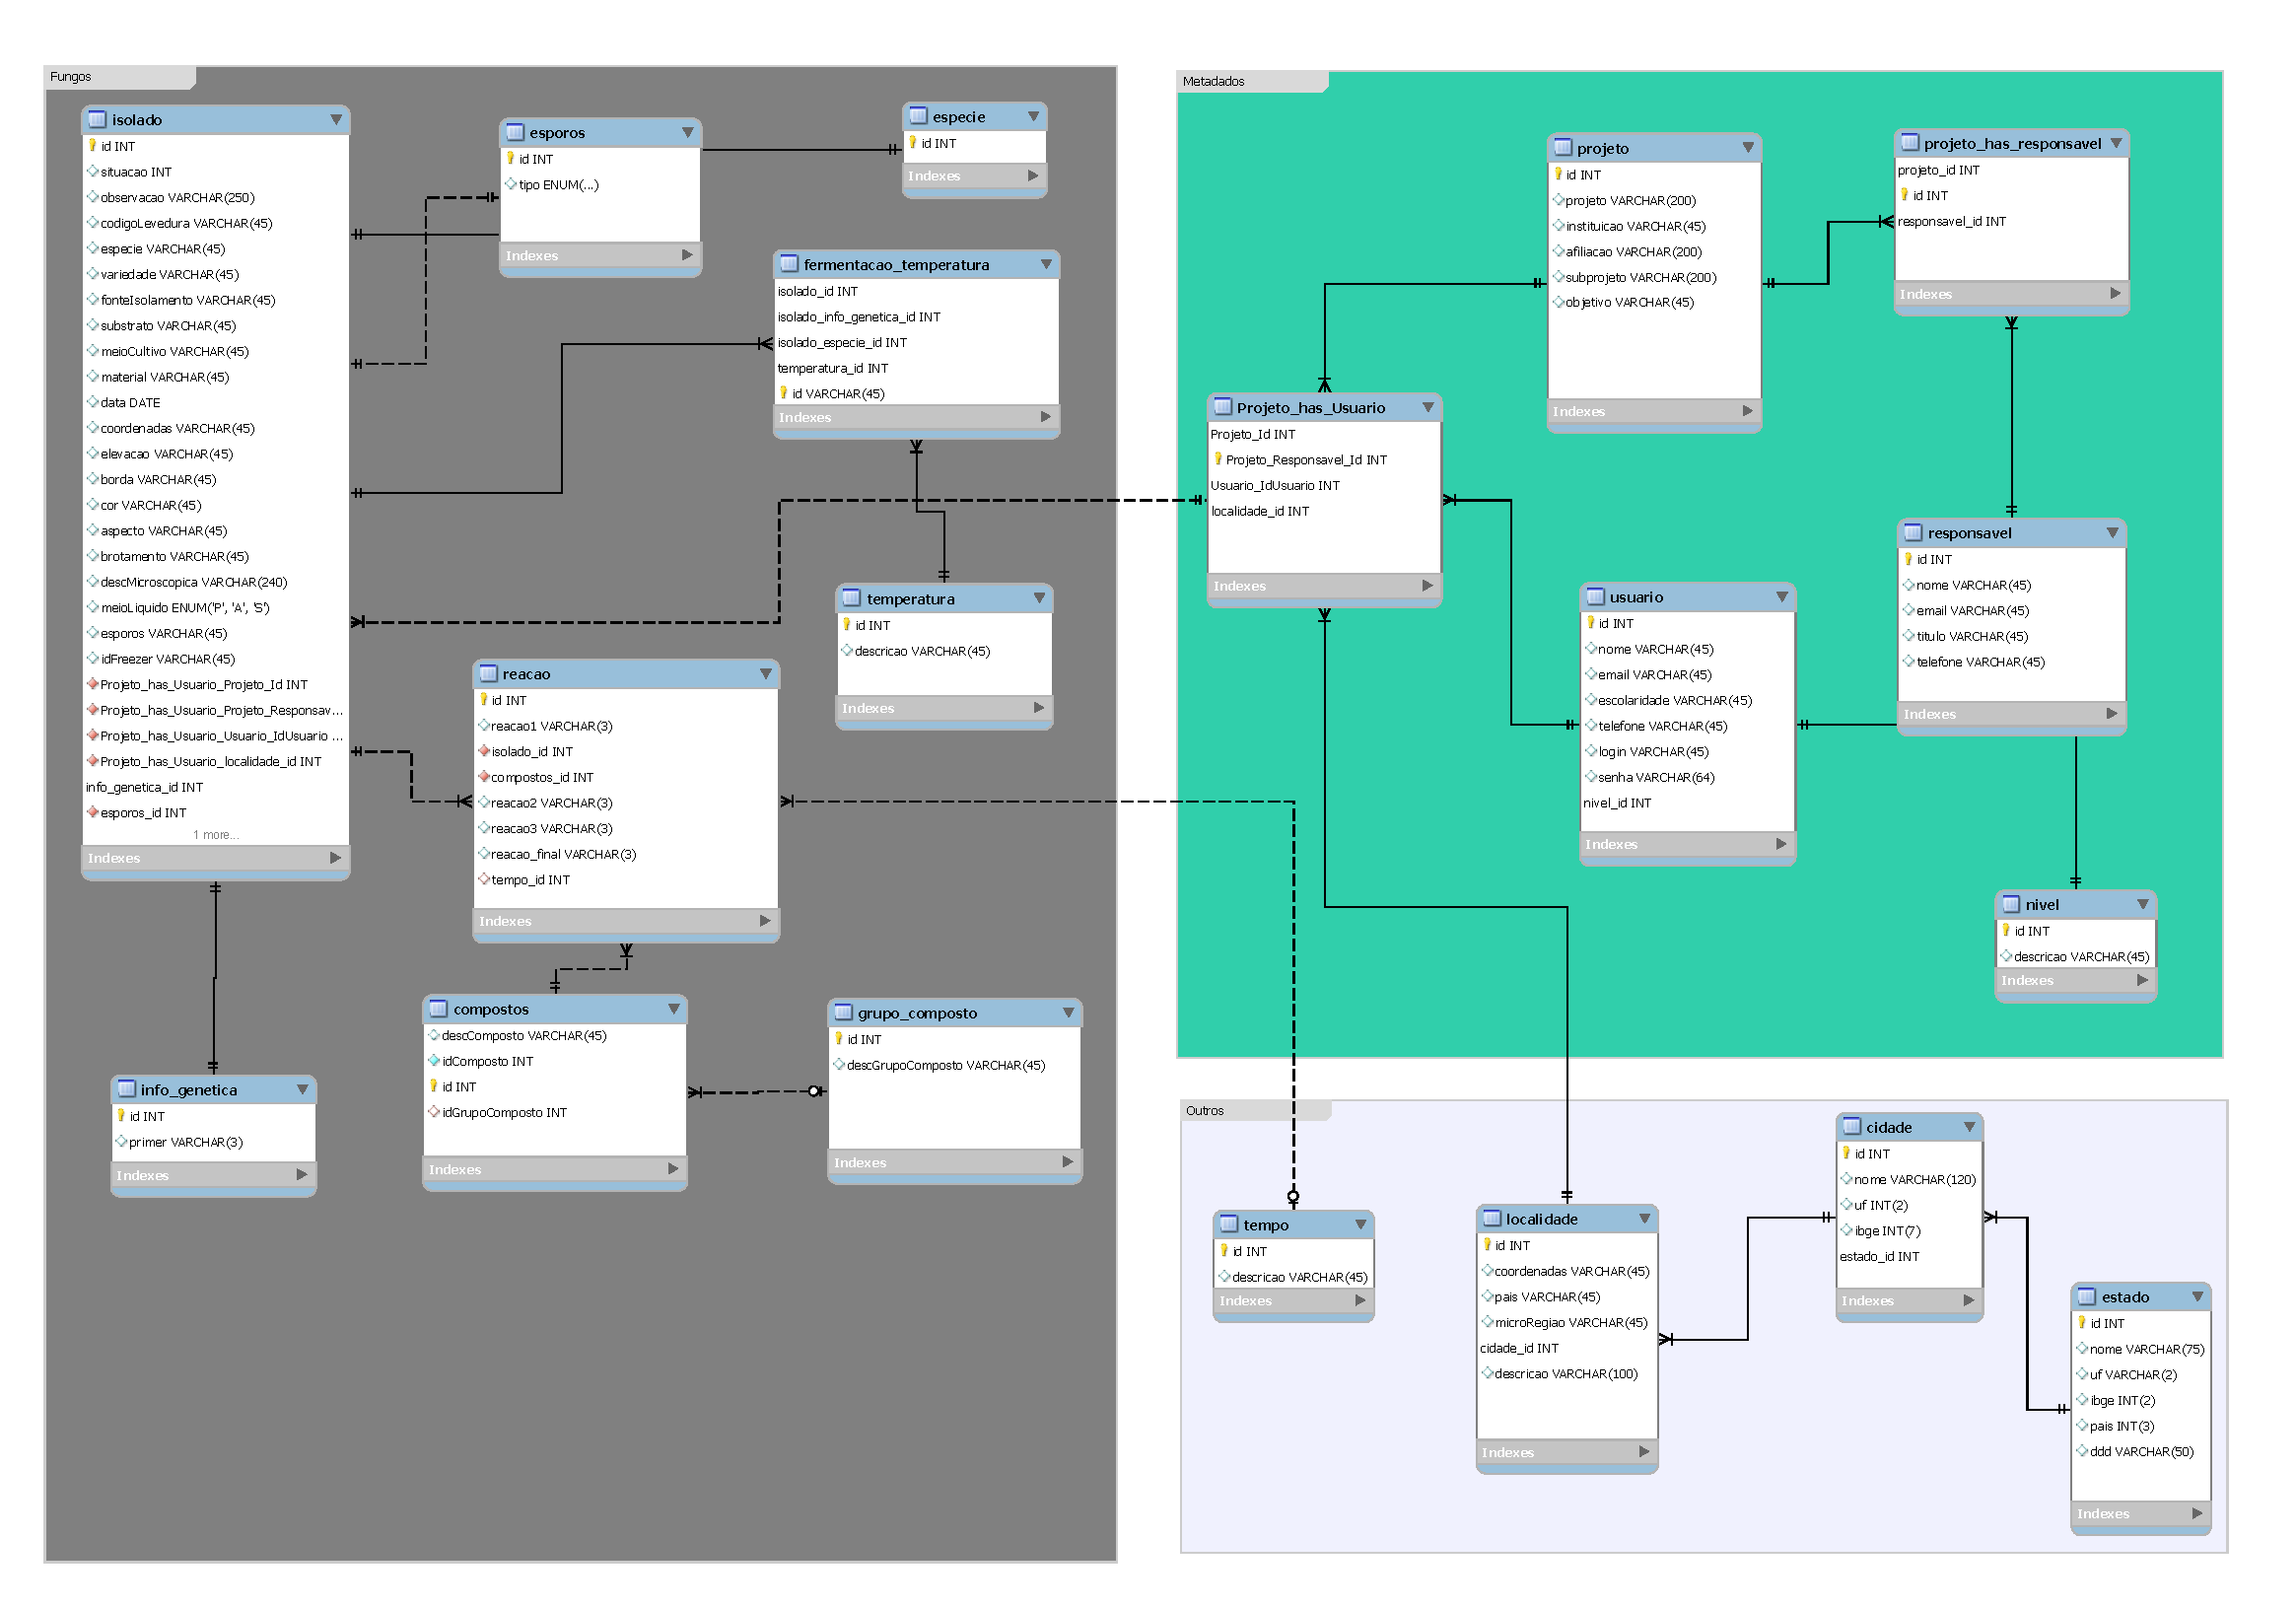
\includegraphics[scale=0.4, angle=270]{TCC_Johnny/pdf/modelo_ER.pdf}
      \label{ape:modeloER}
      \caption{Proposta de Modelo Entidade Relacionamento}
       \raggedright \scriptsize \centering  Fonte: do Autor
    \end{figure}% TODO: aguardando dados do especialista para conclusão dos relacionamentos das entidades apresentadas.

\chapter{Fichas de catalogação de culturas}
\label{ape:fichas}

\begin{figure}[ht]
    \centering
      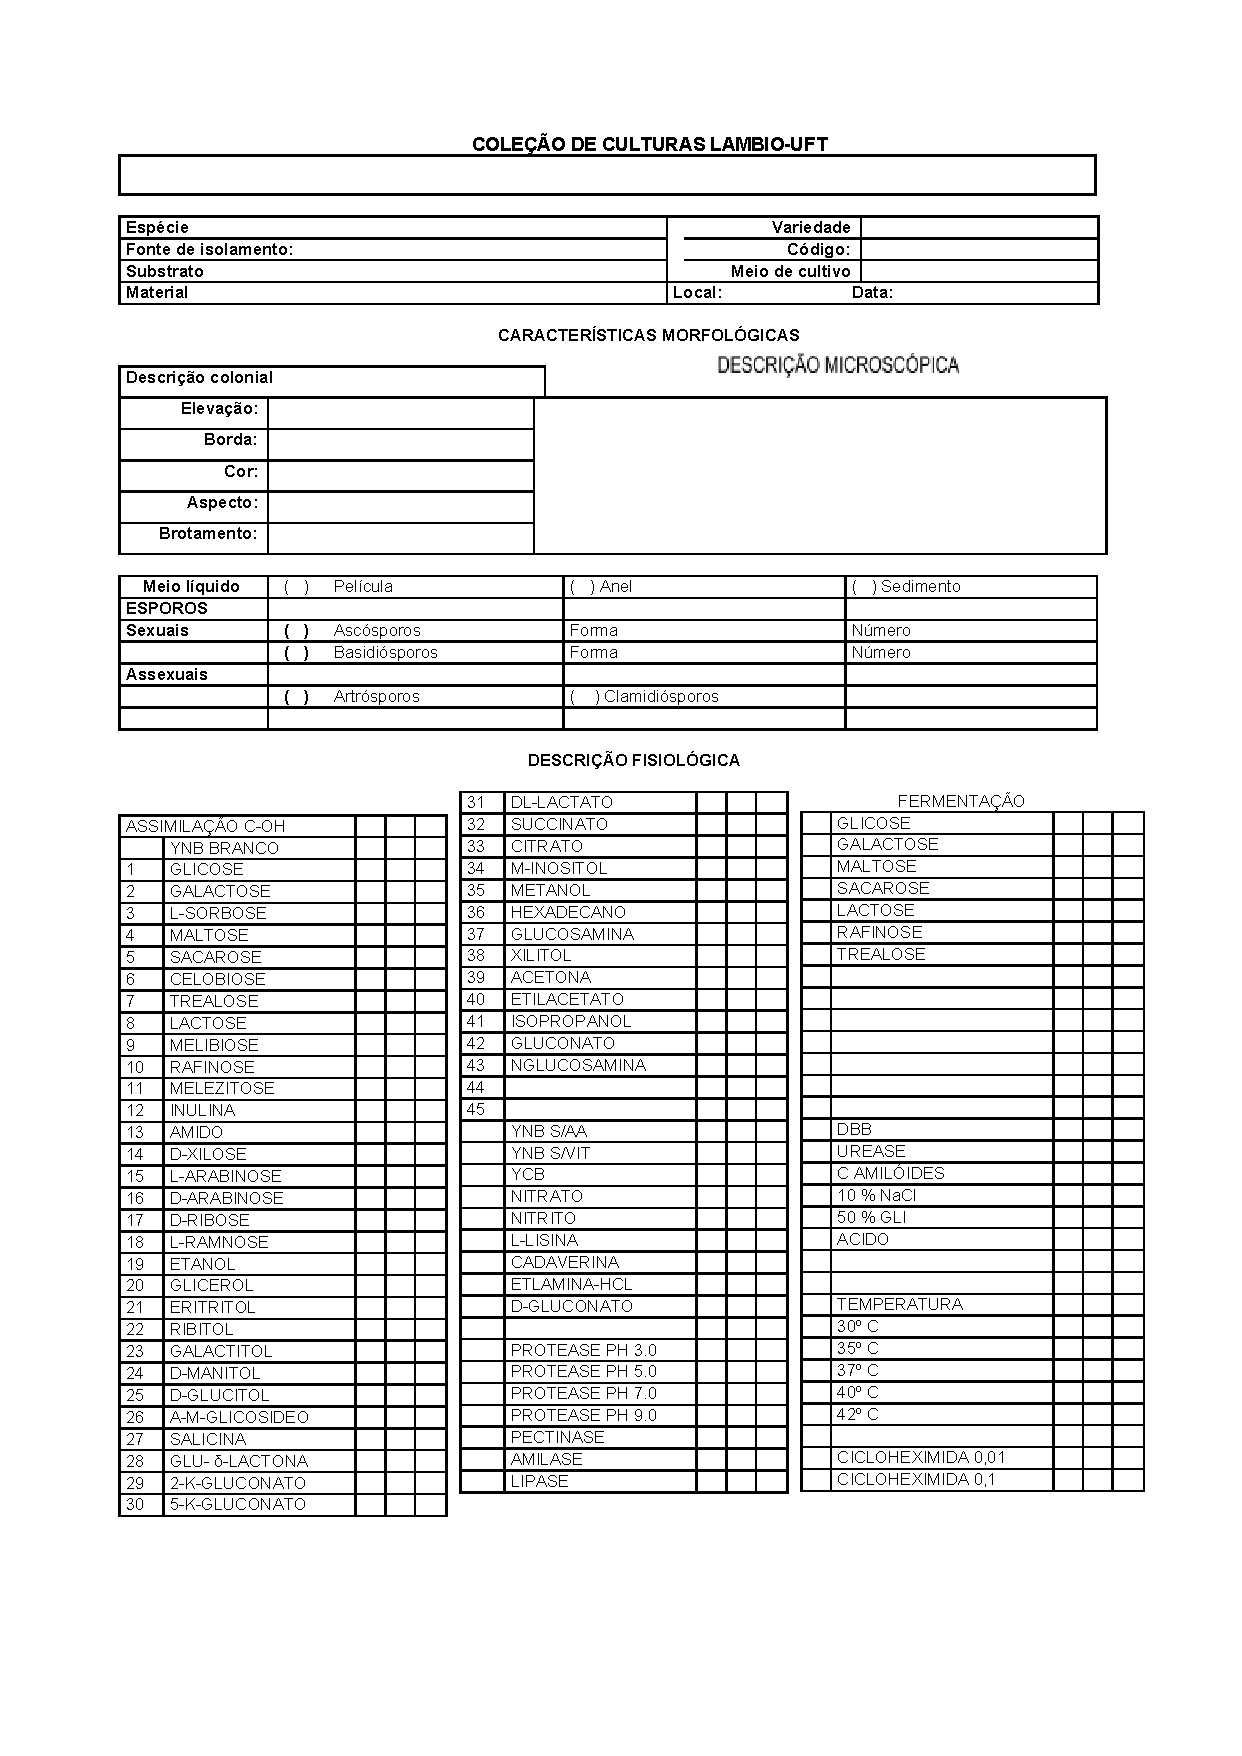
\includegraphics[scale=0.6]{TCC_Johnny/pdf/ficha_Culturas.pdf}
      \label{ape:ficha_culturas}
      \caption{Ficha Coleção de Culturas - LAMBIO/UFT}
       \raggedright \scriptsize \centering  Fonte: LAMBIO/UFT
    \end{figure}%

\begin{figure}[ht]
    \centering
      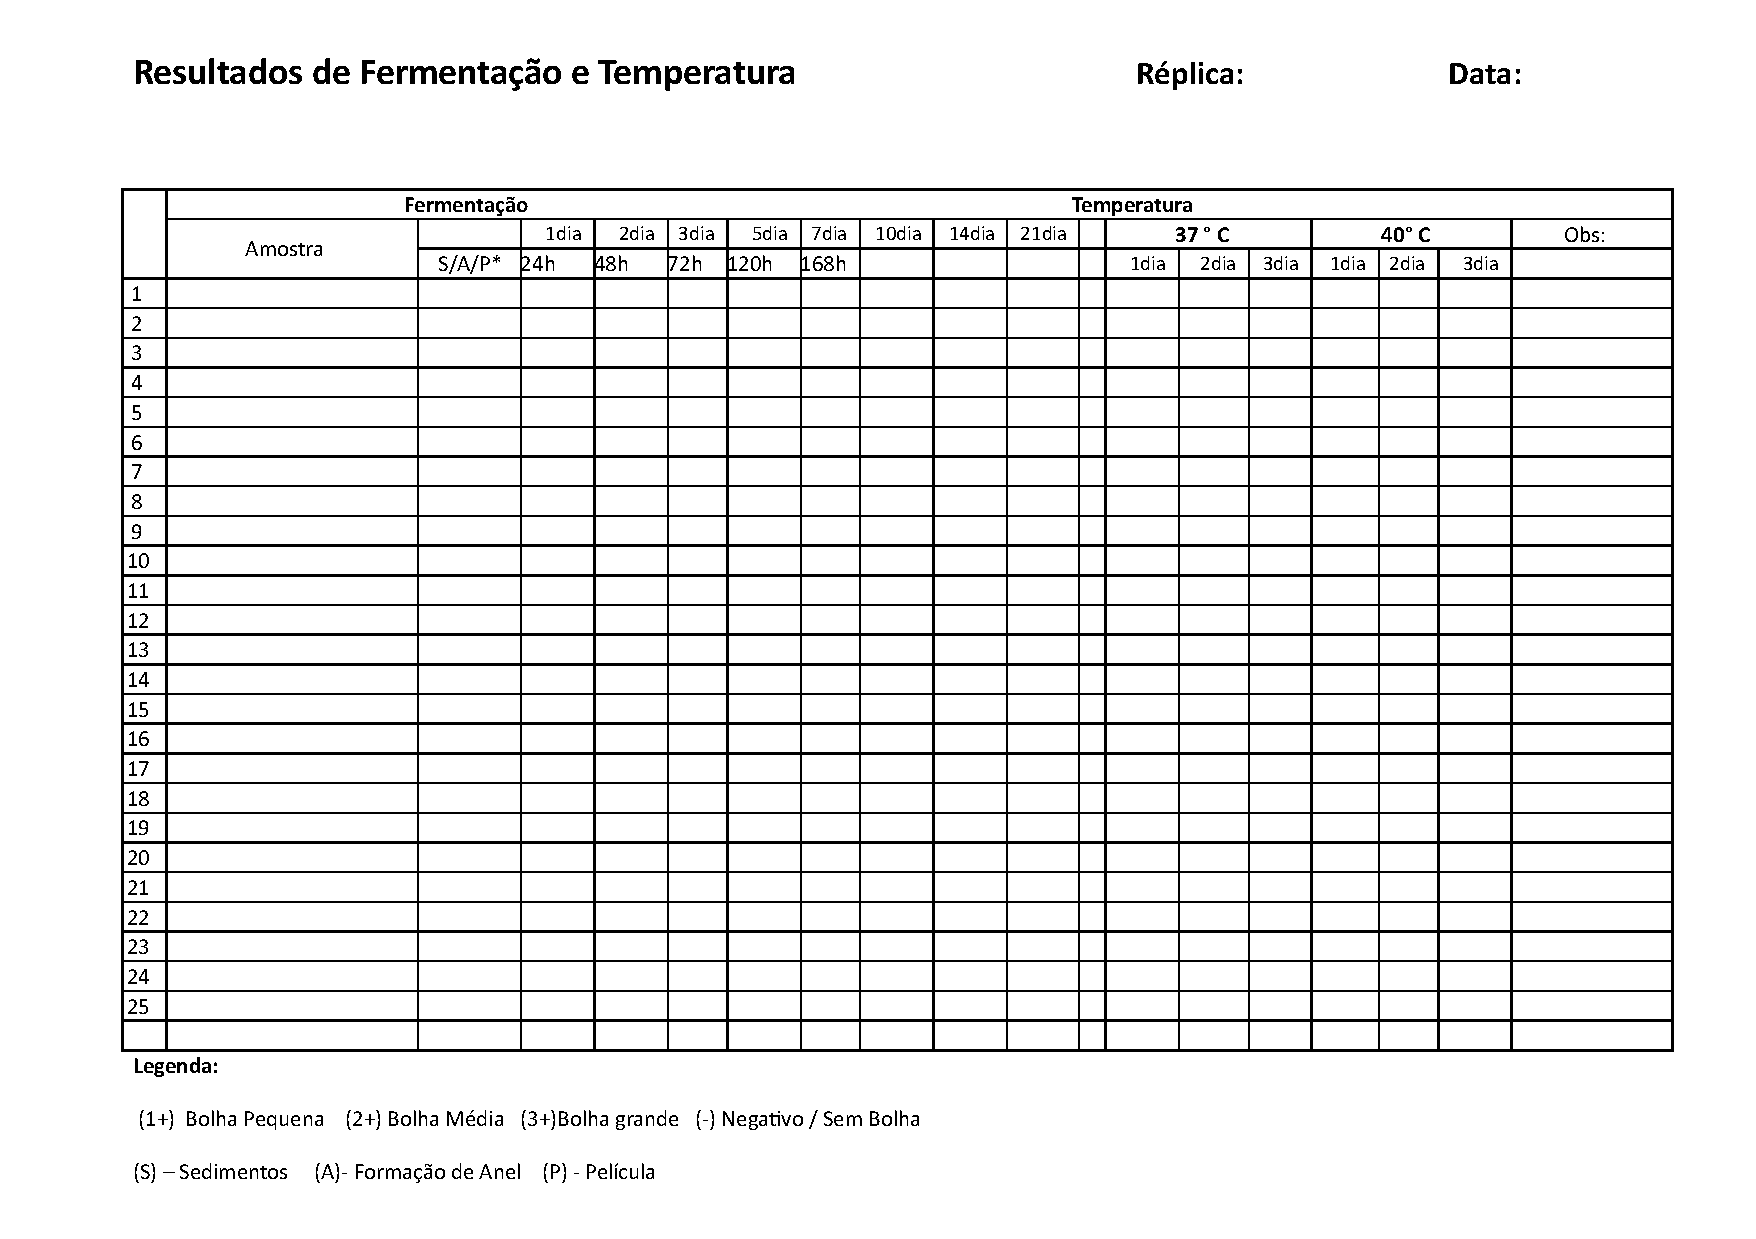
\includegraphics[scale=0.6, angle=270]{TCC_Johnny/pdf/ficha_Fermentacao.pdf}
      \label{ape:ficha_fermentacao}
      \caption{Ficha Resultado Fermentação e Temperatura - LAMBIO/UFT}
       \raggedright \scriptsize \centering  Fonte: LAMBIO/UFT
    \end{figure}%


% TODO: adicionar o Dicionário de Dados aqui

\end{document}
